
\section{Building SMBLD: a new parametric dog model}

% Explain why the SMAL parameteric model is unsuitable for the dog category.

At the heart of the method is a parametric representation of a 3D animal mesh, which is based on the Skinned Multi-Animal Linear (SMAL) model proposed by Zuffi et al.~\cite{zuffi2017menagerie}. As discussed in \Cref{chap:cgas}, SMAL is a deformable 3D quadruped mesh parameterized by shape and pose. The \emph{shape}~$\shape \in \R\nshape$ parameters are PCA coefficients of an undeformed template mesh with limbs in default position. The \emph{pose}~$\pose \in \R\npose$ parameters meanwhile govern the joint angle rotations ($35 \times 3$ Rodrigues parameters) which effect the articulated limb movement. The SMAL generator function can therefore be viewed supplying a set of triangles and a function 
\begin{equation}
\verts(\pose, \shape,) : \R \npose \times \R \nshape \mapsto \RR 3 \nverts
\end{equation}
which generates the set of 3D model vertex positions $\verts(\pose, \shape) \in \RR{3889}{3}$ for the given pose, shape. Also required are a set of position parameters $\posn$ which governs the global orientation and translation of the model. The following represents a 3D model of given pose and shape transformed to its 3D position.

\begin{equation}
    \posn * \verts(\pose, \shape)
\end{equation}    

In addition, the SMAL model 3D joints locations are obtained from the output set of vertcies by post-multiplying by a $\nverts \times \njoints$ matrix $\jointselect$.  The $j^{\text{th}}$ column of~$\jointselect$ defines the 3D position of joint~$j$ as a linear combination of the vertices.

\begin{equation}
J(\pose, \shape, \posn) := \proj(\posn * \verts(\pose, \shape, \posn) \jointselect)
\end{equation}

% model consists of a linear blend skinning function $F_{v}: (\pose, \shape) \mapsto V$, which generates a set of vertex positions $V \in \RR{3889}{3}$, and a joint function $F_{J}: (\pose, \shape) \mapsto J$, which generates a set of joint positions $J \in \RR{35}{3}$.

% TODO: Use consistent notation!
% This section provides a formal definition for the deformable 3D model that is used to generate synthetic training data and in the model fitting stage to obtain the final mesh. Our system assumes a deformable 3D model such as SMAL~\cite{zuffi2017menagerie} which parametrizes a 3D mesh as a function of {\em pose} parameters~$\pose \in \R\npose$ (e.g.\ joint angles) and {\em shape} parameters~$\shape \in \R\nshape$. 
% As discussed in \Cref{chap:relwork}, a 3D mesh is an array of vertices $\verts \in \RR 3\nverts$ (the vertices are columns of a $3 \times \nverts$ matrix) and a set of triangles represented as integer triples $(i,j,k)$, which are indices into the vertex array.
% A deformable model such as SMAL may be viewed as supplying a set of triangles, and a function
% \begin{equation}
% \verts(\pose, \shape) : \R \npose \times \R \nshape \mapsto \RR 3 \nverts
% \end{equation}
% which generates the 3D model for a given pose and shape.
% The mesh topology (i.e.~the triangle vertex indices) is provided by the deformable model, and is the same for all shapes and poses we consider, so in the sequel a mesh will be defined only by the 3D positions of its vertices.

% In any given image, the model's 3D {\em position} (i.e.\ translation and orientation) is also unknown, and will be represented by a parametrization $\posn$ which may be for example translation as a 3-vector and rotation in axis angle form. Application of such a transformation to a $3\times\nverts$ matrix will be denoted by $*$, so that 
% \begin{equation}
% \posn * \verts(\pose, \shape)
% \end{equation}
% represents a 3D model of given pose and shape transformed to its 3D position.


\subsection{Introducing scale parameters}

While SMAL has been shown to be adequate for representing a variety of quadruped types, the modes of dog shape variation are poorly captured by the current model. This is unsurprising, since SMAL used only four dogs in its construction.

This is overcome with a simple but effective way to improve the model's representational power over this particularly diverse animal category. The set of shape parameters $\beta$ are augmented with an additional set $\scale$ which independently scale parts of the mesh. For each model joint, parameters ${\scale_x,\scale_y,\scale_z}$ are defined which apply a local scaling of the mesh along the local coordinate $x, y, z$ axes, before pose is applied. Allowing each joint to scale entirely independently can however lead to unrealistic deformations, so scale parameters are shared between multiple joints, e.g. leg lengths. The new Skinned Multi-Breed Linear Model for Dogs (SMBLD) is therefore adapted from SMAL by adding $6$ scale parameters to the existing set of shape parameters. Figure~\ref{fig:shape_variation} shows how introducing scale parameters increases the flexibility of the SMAL model. The original SMAL shape prior is also extended to cover the new scale parameters by fitting SMBLD to a set of $13$ artist-designed 3D dog meshes. 

\begin{figure*}[t!]
    \centering
    % \includegraphics[width=0.23\linewidth]{OllieFigs/mean.png}
    % \includegraphics[width=0.23\linewidth]{OllieFigs/leg_lengthen.png}
    % \includegraphics[width=0.23\linewidth]{OllieFigs/tail_shorten.png}
    % \includegraphics[width=0.23\linewidth]{OllieFigs/tail_puff.png}
    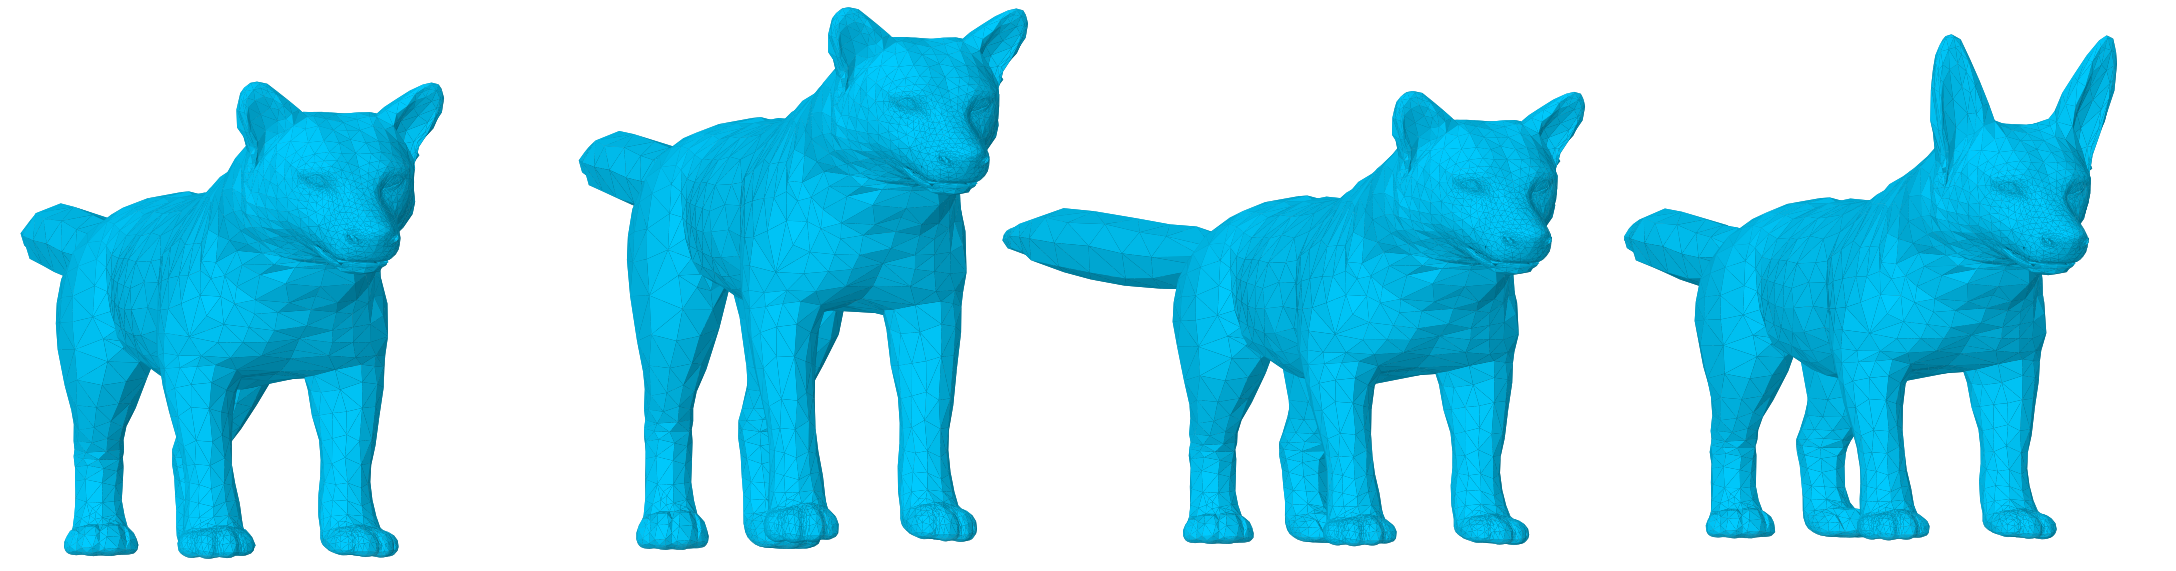
\includegraphics[width=.95\linewidth]{OllieFigs/all_shapevar.png}
    \caption{\textbf{Effect of varying SMBLD scale parameters}. 
    \emph{From left to right}: 
    Mean SMBLD model, 
    25\% leg elongation,
    50\% tail elongation,
    50\% ear elongation.}
    \label{fig:shape_variation}
\end{figure*}

\subsection{Learning a prior over scale parameters}

Next of concern is how to adapt the existing SMAL shape prior to cover the new set of scale parameters and thereby better represent the dog category. This is achieved by fitting SMBLD to a set of $13$ artist-designed 3D dog meshes, designed for animation and which offer more variety than the original set of SMAL toys. An energy minimization process is used to align the SMAL vertices to each scan, under smoothing regularizers. 

\subsubsection{Preliminaries: the SMAL shape prior}
For shape spaces shape space formulations based on principal component analysis (PCA), recall the linear generator function $g: \R{d} \mapsto \R{3n}$ which maps a $d$-dimensional parameter space to $n$ 3D morphable model vertex coordinates: 

\begin{equation}
    g(w) = \bar{c} + Ew
\end{equation}

In this formulation, $\bar{c} \in \R{3n}$ is the mean 3D shape from a training dataset, and $E \in \R{3n \times d}$ is a matrix containing the $d$ most dominant eigenvectors computed over shape residuals $\{c_i - \bar{c_i}\}$. 

% Another hypothesis is that the 3D faces in the reduced parameter space R
% d follow a multivariate normal distribution, which can be directly deduced from the eigenvalues corresponding to E.

%% PCA does assumlaxe normal distribution of features See p.55 SAS book1 or Rummel, 19702 or Mardia, 19793.

A consequence of PCA construction is that the features in the $d$-dimensional parameter space follow a multivariate normal distribution. This can be directly derived from the eigenvalues corresponding to $E$. %% ASK ANDREW, or be less lazy and do the math
With this construction, one can define a likelihood function which measures the probability of a given shape vector $w \in \R{d}$

\begin{equation}
    f(w) = (2\pi)^{-\frac{d}{2}}\det(\Sigma)^{-\frac{1}{2}}e^{-\frac{1}{2}(w-\bar{c})^T\Sigma^{-1}(w-\bar{c})}
\end{equation}

For problems which aim to optimize $w$, the 3D shape prior is obtained by maximizing $f(w)$ or equivalently, by minimizing the negative log likelihood

\begin{equation}
     -\ln\left[f(w)\right] = -\frac{1}{2}\left[\ln\det(\Sigma) + d\ln(2\pi) +  (w - \bar{c})^T\Sigma^{-1}(w-\bar{c})\right]
\end{equation}
and dropping terms with no dependency on $w$ (which remain constant during optimization) leaves the Mahalanobis distance of $w$ to the origin

\begin{equation}
    L(w) = (w - \bar{c})^T\Sigma^{-1}(w-\bar{c})
\end{equation}

% END PRELIMINARIES

% We have already seeen this formulation in Chapter 4.

\subsubsection{Learning an improved prior via 3D model fitting}

Recall that SMBLD is adapted from the SMAL~\cite{zuffi2017menagerie} deformable animal mesh, by including limb scaling parameters. A new shape prior is learnt by fitting this new SMBLD model, which comprises parameters for pose $\pose$ and shape $\beta$ (the latter of which now includes scaling parameters $\kappa$).

Note that fitting SMBLD to 3D scans emits much simpler optimization than to 2D images, since the complete 3D information of the target mesh is available. In addition, the target meshes are not particularly detailed and are already aligned in the canonical T-pose, so we avoid need for a complex alignment technique as discussed in \Cref{chap:cgas}. 

An energy minimization process is used to align the SMBLD mesh to the 3D scans, subject to some smoothing regularizers. The following energy formulation is minimized

\begin{equation}
    \E{opt} = \E{chamfer} + \E{laplacian} + \E{edge} + \E{normal}
\end{equation}
where each of these terms has a scalar weight $\lambda$. Here, $\W{chamfer}=\W{edge}=1.0$, $\W{normal}=0.01$ and $\W{laplacian}=0.1$. Optimization is run using stochastic gradient descent (SGD) with learning rate $1.0e^{-4}$ for $1000$ iterations. Further details on the specific energy terms are now provided.

\ss{Chamfer energy.} A measure of the average distance between vertices of the SMBLD mesh $V=F_v(\pose, \shape)$, and the target mesh vertices $V'$, when $p$ vertices $v_{i}, v'_{j}$ are sampled from each mesh respectively:
\begin{equation}
        \E{chamfer}(V, V') = \frac{1}{p} \sum_{i=1}^p \min_j^p  \left | v_{i} - v'_{j} \right |
\end{equation}

\ss{Uniform laplacian energy.} A measure of the mesh smoothness.

\ss{Edge energy.} This energy is equal to the average edge length across the mesh, and is used to encourage uniform distribution of vertices.

\ss{Normal energy.} This energy promotes consistency between adjacent faces. It is a measure of the average normal consistency between adjacent faces. For two faces with normals $\mathbf{n_0}$ and $\mathbf{n_1}$, the normal consistency is $1 - \frac{\mathbf{n_0} \cdot \mathbf{n_1}}{\left|\mathbf{n_0}\right|\left|\mathbf{n_1}\right|}$.

At the end of this process, we have a collection of fits $\left|(\pose,\shape)\right|_{\{i=1,...13\}}$ from which we can learn our unimodal pose and shape priors. As discussed, we evenutally use this unimodal shape prior to initialize our mixture shape prior, which is tuned with the expectation-maximization step in the training loop.

% \section{Learning mixture shape prior.}
% This section contains additional detail for how we learn our mixture shape prior, using expectation maximization in-the-loop.


% Way more here, and include exampels